\documentclass[presentation]{beamer}

\usepackage{tikz}
\usetikzlibrary{calc,intersections}
\newsavebox\myAnim

\usepackage{pgfplots}
\pgfplotsset{plot coordinates/math parser=false}

\usepackage{animate}
\usepackage[utf8]{inputenc}
\usepackage[T1]{fontenc}
\usepackage{fixltx2e}
\usepackage{graphicx}
\usepackage{longtable}
\usepackage{float}
\usepackage{wrapfig}
\usepackage{rotating}
\usepackage[normalem]{ulem}
\usepackage{amsmath}
\usepackage{textcomp}
\usepackage{marvosym}
\usepackage{wasysym}
\usepackage{amssymb}
\usepackage{hyperref}
\usepackage{setspace}
\tolerance=1000
\usepackage{graphicx} \DeclareMathOperator{\argmin}{argmin}
\linespread{1}

\newcommand{\me}{\mathrm{e}}
\providecommand{\e}[1]{\ensuremath{\times 10^{#1}}} 
\providecommand{\mb}[1]{\mathbf{#1}}
\providecommand{\mf}[1]{\mathfrak{#1}}
\providecommand{\ro}[1]{\mathbf{\mathfrak{r}}_o}
\providecommand{\so}[1]{\mathbf{\hat{s}}_o}
\providecommand{\rb}[1]{\mathbf{r}_b}
\providecommand{\rbm}[1]{r_b^{\text{m}}}
\providecommand{\rd}[1]{\mathbf{r}_d}
\providecommand{\mh}[1]{\mathbf{\hat{#1}}}
\providecommand{\bs}[1]{\boldsymbol{#1}} 
\providecommand{\intinf}{\int_{-\infty}^{\infty}}
\newcommand{\under}[2]{\underset{\scriptscriptstyle#1}{#2}}

\usetheme{simple} \usecolortheme{} \usefonttheme{serif} \useinnertheme{}
\useoutertheme{}

\begin{document}
\begin{frame}{
    \vspace{0em}
    \begin{center}
      Live-Cell Biology with Three-Dimensional\\
      Fluorescence Orientation Microscopy
    \end{center}}
  \vspace{-2em}
  \centering
  \animategraphics[loop, autoplay, palindrome, width=0.65\linewidth, controls, buttonsize=0.5em]{10}{figs/recon/}{1}{160}
  \begin{center}
    \vspace{0em}
    Talon Chandler\\ \vspace{0.5em}
  March 21, 2018
  \end{center}
\end{frame}

\begin{frame}
  \begin{columns}[totalwidth=6cm]
    \begin{column}{.5\textwidth}
      \centering
      \onslide<1->{\textbf{PET/SPECT}}\\ \vspace{0.2em}
      \onslide<1->{\centering \includegraphics[width=0.35\textwidth]{figs/spect.png}}\\
      % Wong, 2017      
      \onslide<1->{Radionuclide}\\
      \onslide<1->{Human scale}\\
      \onslide<1->{Medical discovery}\\
    \end{column}
    \begin{column}{.5\textwidth}
      \centering
      \onslide<2->{\textbf{Fluorescence Microscopy}}\\ \vspace{0.2em}
      \onslide<2->{\centering \includegraphics[width=0.52\textwidth]{figs/cellinv.jpg}}\\
      %Iacoviello, 1995
      \onslide<2->{Fluorophore}\\
      \onslide<2->{Cell scale}\\
      \onslide<2->{Biological discovery}\\
    \end{column}
  \end{columns}
  \centering
  \vspace{2em}
  \onslide<3->{\textbf{Improve human lives}}
\end{frame}

\begin{frame}{Three parts}
  
\end{frame}

\begin{frame}[label=sec-1]{Part 1: Position}
 \begin{center}
   \includegraphics[width=0.8\textwidth]{figs/bee1.jpg}
%http://mediad.publicbroadcasting.net/p/wnmu/files/styles/x_large/public/201712/bee.jpg
 \end{center}
\end{frame}

\begin{frame}{Microscope animation slide}
  
\end{frame}

\begin{frame}{Where can we find fluorescent samples?} 
  \begin{columns}
    \begin{column}{.33\textwidth}
      \centering
      \onslide<1->{\textbf{Endogenous}}\\ \vspace{0.2em}
      \onslide<1->{\centering \includegraphics[width=1.0\textwidth]{figs/aequoria.jpg}}\\
      %http://lem.ch.unito.it/didattica/infochimica/2008_GFP/estrazione.html
    \end{column}
    \begin{column}{.33\textwidth}
      \centering
      \onslide<3->{\textbf{Genetic}}\\ \vspace{0.2em}
      \onslide<3->{\centering \includegraphics[width=1.0\textwidth]{figs/GFP_mouse.jpg}}\\
      %http://sites.udel.edu/art-in-science/2016/02/18/green-fluorescent-protein-illuminating-molecular-level-processes/
    \end{column}
    \begin{column}{.33\textwidth}
      \centering
      \onslide<2->{\textbf{Exogeneous}}\\ \vspace{0.2em}
      \onslide<2->{\centering \includegraphics[width=1.0\textwidth]{figs/dyes.jpg}}\\
      % http://www.healthfreedoms.org/fluorescent-dyes-light-up-brain-cancer-cells/
    \end{column}
  \end{columns}
\end{frame}

\begin{frame}{What data do we collect?}
  Intensities. 
\end{frame}

\begin{frame}{What can we study?}
  Examples x3
\end{frame}

\begin{frame}{Review}
  Biological question -> fluorescent label -> ***microscopic imaging*** ->
  biological conclusion
\end{frame}

\begin{frame}[label=sec-1]{Part 2: Orientation}
 \begin{center}
   \includegraphics[width=0.8\textwidth]{figs/bee2.jpg}
%https://www.thoughtco.com/how-to-save-the-worlds-bees-1140836
 \end{center}
\end{frame}

\begin{frame}{Redo microscope slide}
  
\end{frame}

\begin{frame}{\centering Monopole $\neq$ Dipole}
  \vspace{1em}
  \begin{columns}
    \begin{column}{.5\textwidth}
      \centering Monopole emitter \\ \vspace{.5em}
    \animategraphics[autoplay, loop, width=1.\textwidth]{10}{figs/monopole/monopole}{}{}  
  \end{column}
  \begin{column}{.5\textwidth}
    \centering Dipole emitter \\ \vspace{.5em}
    \animategraphics[autoplay, loop, width=1.\textwidth]{10}{figs/dipole/dipole}{}{}  
  \end{column}    
\end{columns}
\centering
\vspace{0.5em}
\pause
\rotatebox{180}{\Huge {$\curvearrowright$}}\\ \vspace{0.5em}
quickly rotating fluorophores\\
or\\
many fluorophores in all orientations \\
\end{frame}  

\begin{frame}{Polarized Light}
\begin{center}
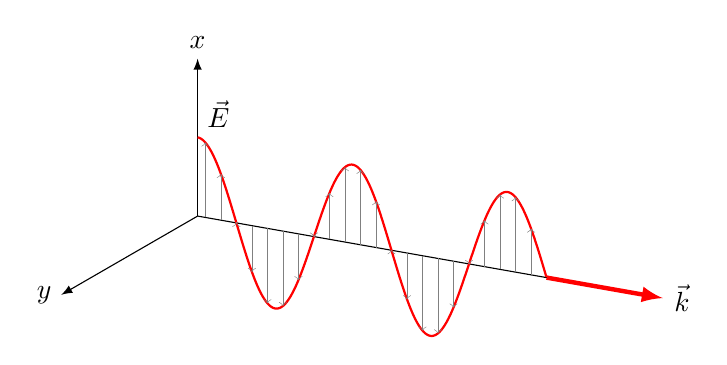
\begin{tikzpicture}[x={(-10:1cm)},y={(90:1cm)},z={(210:1cm)}]
    % Axes
    \draw (0,0,0) node[above]{} -- (5,0,0) {};
    \draw[-latex] (0,0,0) -- (0,2,0) node[above] {$x$};
    \draw[-latex] (0,0,0) -- (0,0,2) node[left] {$y$};
    \draw[-latex, ultra thick, red] (4.5,0,0) -- (6,0,0) node[right, black] {$\vec{k}$} ;
    % Waves
    \draw[thick, red] plot[domain=0:4.5,samples=200] (\x,{cos(deg(pi*\x))},0);
    %\draw[white,thick] plot[domain=0:4.5,samples=200] (\x,0,{cos(deg(pi*\x))});
    % Arrows
    \foreach \x in {0.1,0.3,...,4.4} {
      \draw[->,help lines] (\x,0,0) -- (\x,{cos(deg(pi*\x))},0);
    %  \draw[->,help lines] (\x,0,0) -- (\x,0,{cos(deg(pi*\x))});
    }
    % Labels
    \node[above right] at (0,1,0) {$\vec{E}$};
  \end{tikzpicture}
  \end{center}
\end{frame}

\begin{frame}{Polarized Light}
\begin{center}
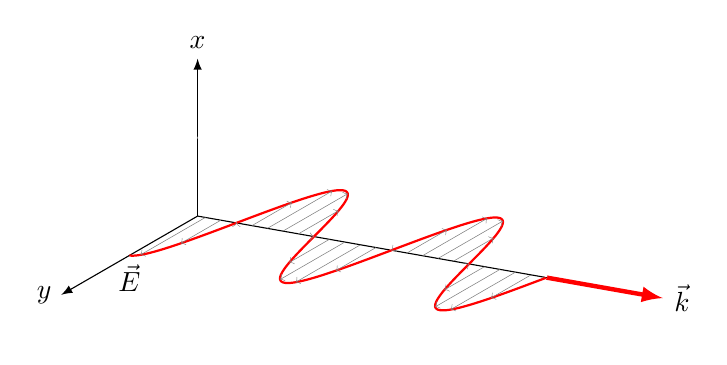
\begin{tikzpicture}[x={(-10:1cm)},y={(90:1cm)},z={(210:1cm)}]
    % Axes
    \draw (0,0,0) node[above] {} -- (5,0,0) {};
    \draw[-latex] (0,0,0) -- (0,2,0) node[above] {$x$};
    \draw[-latex] (0,0,0) -- (0,0,2) node[left] {$y$};
    \draw[-latex, ultra thick, red] (4.5,0,0) -- (6,0,0) node[right, black] {$\vec{k}$} ;
    % Waves
    \draw[white, thick] plot[domain=0:4.5,samples=200] (\x,{cos(deg(pi*\x))},0);
     \draw[thick, red] plot[domain=0:4.5,samples=200] (\x,0,{cos(deg(pi*\x))});
    % Arrows
    \foreach \x in {0.1,0.3,...,4.4} {
      \draw[->,help lines] (\x,0,0) -- (\x,0,{cos(deg(pi*\x))});
    }
    % Labels
    \node[below] at (0,0,1) {$\vec{E}$};
  \end{tikzpicture}
  \end{center}
\end{frame}


\begin{frame}{Monopole vs. dipole excitationn}
    Animation
    In the limit
\end{frame}

\begin{frame}{Three ways to measure the dipole moment}
    In the limit
\end{frame}

\begin{frame}[label=sec-1]{Part 3: Proposal}
 \begin{center}
   \includegraphics[width=0.8\textwidth]{figs/bee3.jpg}
%https://www.bee-america.com/content/5-things-about-bees-will-amaze-you
 \end{center}
\end{frame}


\end{document}